\section{Einleitung}
Einleitung


\begin{longtable}{|p{5cm}|p{3cm}|p{3.5cm}|p{3cm}|}
\hline
\textbf{Frage} & \textbf{Antwort-Algorithmuszeit (ns)} & \textbf{Transkriptionszeit (ns)} & \textbf{Gesamtzeit (ns)} \\
\hline
\endfirsthead

\hline
\textbf{Frage} & \textbf{Antwort-Algorithmuszeit (ns)} & \textbf{Transkriptionszeit (ns)} & \textbf{Gesamtzeit (ns)} \\
\hline
\endhead

\hline
\endfoot

Wie oft muss man einen PTB schreiben? & 33659000 & 2432785000 & 2474059000 \\
\hline

\end{longtable}

\textbf{Durchschnittszeiten:}
\begin{itemize}
    \item Antwort-Algorithmuszeit: 17228100 ns
\end{itemize}

\subsubsection{Beschreibung}
\ac{knowlegdeGraphs} stellen eine strukturierte Darstellungsform von Informationen dar, welche aus unstrukturierten Texten gewonnen werden. Sie setzen sich aus Informationsentätiten, welche Knoten genannt werden, und Beziehungen zwischen den Informationsentätiten, welche Kanten genannt werden, zusammen. Diese werden aus Textdaten abgeleitet. Dadurch wird die Integration, der Abruf und die Analyse von Informationen erleichtert \cite{Hojas-Mazo2018A}. Um einen KG aus einem Text zu konstruieren, werden verschiedene Methoden. Beispiele dafür sind Techniken wie \ac{OpenIE}, \ac{ML} und semantische Analyse zum Einsatz \cite{OpenIEbased}.

\begin{center}% 'h'
    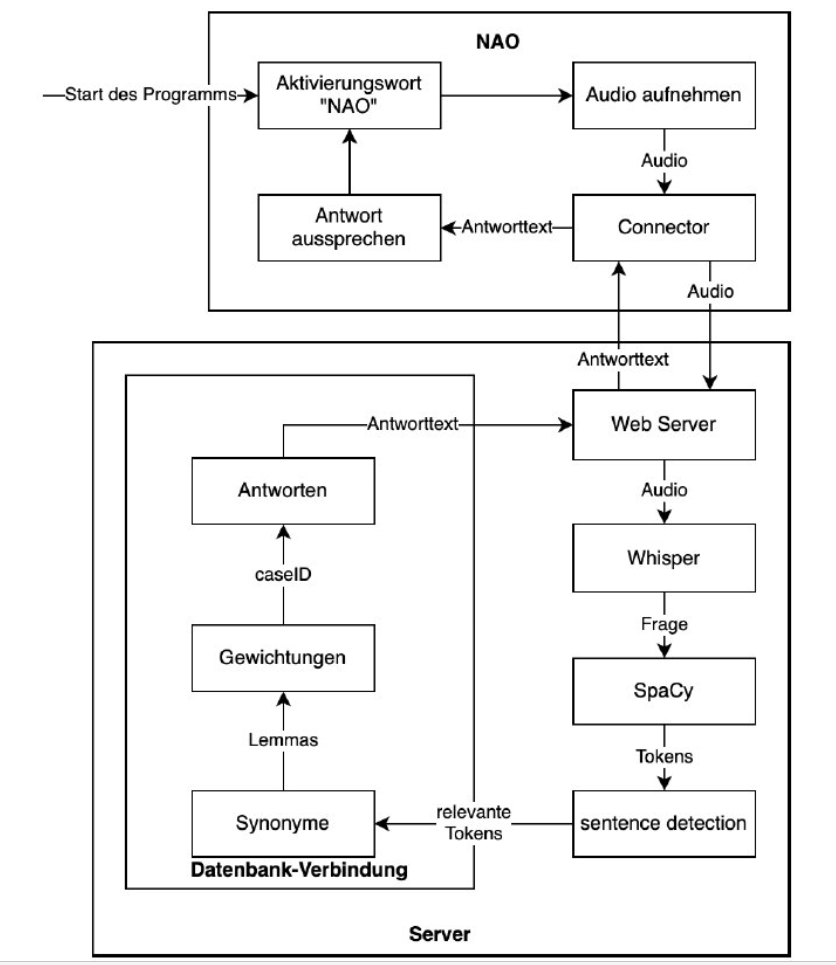
\includegraphics[width=9cm,keepaspectratio]{images/bisherigesProgramm.png}
    \captionof{figure}{Bild1}
    \label{bildReferenz}
\end{center}


% Kommentar1%


\begin{enumerate}
    \item \textbf{Fett 1} Nummerierte liste 1
    \item \textit{Kursiv 1} Nummerierte liste 1
\end{enumerate}


Eine Matheformel (Satz des Pythagoras):

\[
a^2 + b^2 = c^2
\]

wobei \(a\) und \(b\) die Längen der Katheten eines rechtwinkligen Dreiecks sind, und \(c\) die Länge der Hypotenuse.



\begin{lstlisting}[caption={Pip Update}, label={lst:upgradePip}]
    Python Code Section 1
\end{lstlisting}


'''Deutsche Anführungszeichen''' \ref{label1} referenz Zu Label1 
„Anführungszeichen unten, Anführungszeichen oben“

\ref{bildReferenz} Bild Referenz

\newpage
